\clearpage 
\section{Further details on background estimation}
\label{App:FakeLep}
	
	
%%%%
\par{\bf Fake electron sources close to the signal regions \\}
Fig~\ref{Fig:truthComposition_EL_by_source_vs_pt_MORE} shows the number of events and the associated statistical uncertainties for the different fake electrons, for different $p_T$ cuts, in the relaxed signal regions defined in Table~\ref{tab:TruthComposition_SR}. 

Truth composition as a function of fake electron $\eta$, \meff and \met are shown in Fig~\ref{Fig:truthComposition_EL_by_source_vs_eta_MORE}-\ref{Fig:truthComposition_EL_by_source_vs_met_MORE}.

\begin{figure}[p]  
\centering
\subfigure[Baseline electrons, ``relaxed'' SR0b]
{\includegraphics[width=0.49\textwidth]{Truth_Composition/Baseline/NR_Vj_1EL_pT_Var_DEF4.pdf}}
\subfigure[Signal electrons, ``relaxed'' SR0b]{
\includegraphics[width=0.49\textwidth]{Truth_Composition/Signal/NR_Vj_1EL_pT_Var_DEF4.pdf}
}
\subfigure[Baseline electrons, ``relaxed'' SR1b]
{\includegraphics[width=0.49\textwidth]{Truth_Composition/Baseline/NR_Vj_1EL_pT_Var_DEF5.pdf}}
\subfigure[Signal electrons, ``relaxed'' SR1b]{
\includegraphics[width=0.49\textwidth]{Truth_Composition/Signal/NR_Vj_1EL_pT_Var_DEF5.pdf}
}
\subfigure[Baseline electrons, ``relaxed'' SR2b]
{\includegraphics[width=0.49\textwidth]{Truth_Composition/Baseline/NR_Vj_1EL_pT_Var_DEF6.pdf}}
\subfigure[Signal electrons, ``relaxed'' SR2b]{
\includegraphics[width=0.49\textwidth]{Truth_Composition/Signal/NR_Vj_1EL_pT_Var_DEF6.pdf}
} 
\caption   
{Sources of fake electrons as a function of the electron $p_T$, as predicted by MC simulations (combined $t\bar t$ and $V+$ jets) 
in the relaxed signal regions defined in Table~\ref{tab:TruthComposition_SR}. The results are shown for baseline (left) or signal electrons (right). Only the statistical uncertainty are shown.}
\label{Fig:truthComposition_EL_by_source_vs_pt_MORE}
\end{figure}  
	
	
\begin{figure}[p]
\centering
\subfigure[Baseline electrons, ``relaxed'' SR0b]
{\includegraphics[width=0.49\textwidth]{Truth_Composition/Baseline/Vj_1EL_pt15_eta_Var_DEF4.pdf}}
\subfigure[Signal electrons, ``relaxed'' SR0b]{
\includegraphics[width=0.49\textwidth]{Truth_Composition/Signal/Vj_1EL_pt15_eta_Var_DEF4.pdf}
}
\subfigure[Baseline electrons, ``relaxed'' SR1b]
{\includegraphics[width=0.49\textwidth]{Truth_Composition/Baseline/Vj_1EL_pt15_eta_Var_DEF5.pdf}}
\subfigure[Signal electrons, ``relaxed'' SR1b]{
\includegraphics[width=0.49\textwidth]{Truth_Composition/Signal/Vj_1EL_pt15_eta_Var_DEF5.pdf}
}
\subfigure[Baseline electrons, ``relaxed'' SR2b]
{\includegraphics[width=0.49\textwidth]{Truth_Composition/Baseline/Vj_1EL_pt15_eta_Var_DEF6.pdf}}
\subfigure[Signal electrons, ``relaxed'' SR2b]{
\includegraphics[width=0.49\textwidth]{Truth_Composition/Signal/Vj_1EL_pt15_eta_Var_DEF6.pdf}
}
\caption
{Sources of fake electrons as a function of the electron $\eta$, as predicted by MC simulations (combined $t\bar t$ and $V+$ jets) 
in the relaxed signal regions defined in Table~\ref{tab:TruthComposition_SR}. The results are shown for baseline (left) or signal electrons (right).}
\label{Fig:truthComposition_EL_by_source_vs_eta_MORE}
\end{figure} 
%%
\begin{figure}[p]
\centering
\subfigure[Baseline electrons, ``relaxed'' SR0b]
{\includegraphics[width=0.49\textwidth]{Truth_Composition/Baseline/Vj_1EL_pt15_meff_Var_DEF4.pdf}}
\subfigure[Signal electrons, ``relaxed'' SR0b]{
\includegraphics[width=0.49\textwidth]{Truth_Composition/Signal/Vj_1EL_pt15_meff_Var_DEF4.pdf}
}
\subfigure[Baseline electrons, ``relaxed'' SR1b]
{\includegraphics[width=0.49\textwidth]{Truth_Composition/Baseline/Vj_1EL_pt15_meff_Var_DEF5.pdf}}
\subfigure[Signal electrons, ``relaxed'' SR1b]{
\includegraphics[width=0.49\textwidth]{Truth_Composition/Signal/Vj_1EL_pt15_meff_Var_DEF5.pdf}
}
\subfigure[Baseline electrons, ``relaxed'' SR2b]
{\includegraphics[width=0.49\textwidth]{Truth_Composition/Baseline/Vj_1EL_pt15_meff_Var_DEF6.pdf}}
\subfigure[Signal electrons, ``relaxed'' SR2b]{
\includegraphics[width=0.49\textwidth]{Truth_Composition/Signal/Vj_1EL_pt15_meff_Var_DEF6.pdf}
}
\caption
{Sources of fake electrons as a function of \meff, as predicted by MC simulations (combined $t\bar t$ and $V+$ jets) 
in the relaxed signal regions defined in Table~\ref{tab:TruthComposition_SR}. The results are shown for baseline (left) or signal electrons (right).}
\label{Fig:truthComposition_EL_by_source_vs_meff_MORE}
\end{figure} 
%%
\begin{figure}[p]
\centering
\subfigure[Baseline electrons, ``relaxed'' SR0b]
{\includegraphics[width=0.49\textwidth]{Truth_Composition/Baseline/Vj_1EL_pt15_met_Var_DEF4.pdf}}
\subfigure[Signal electrons, ``relaxed'' SR0b]{
\includegraphics[width=0.49\textwidth]{Truth_Composition/Signal/Vj_1EL_pt15_met_Var_DEF4.pdf}
}
\subfigure[Baseline electrons, ``relaxed'' SR1b]
{\includegraphics[width=0.49\textwidth]{Truth_Composition/Baseline/Vj_1EL_pt15_met_Var_DEF5.pdf}}
\subfigure[Signal electrons, ``relaxed'' SR1b]{
\includegraphics[width=0.49\textwidth]{Truth_Composition/Signal/Vj_1EL_pt15_met_Var_DEF5.pdf}
}
\subfigure[Baseline electrons, ``relaxed'' SR2b]
{\includegraphics[width=0.49\textwidth]{Truth_Composition/Baseline/Vj_1EL_pt15_met_Var_DEF6.pdf}}
\subfigure[Signal electrons, ``relaxed'' SR2b]{
\includegraphics[width=0.49\textwidth]{Truth_Composition/Signal/Vj_1EL_pt15_met_Var_DEF6.pdf}
}
\caption
{Sources of fake electrons as a function of \met, as predicted by MC simulations (combined $t\bar t$ and $V+$ jets) 
in the relaxed signal regions defined in Table~\ref{tab:TruthComposition_SR}. The results are shown for baseline (left) or signal electrons (right).}
\label{Fig:truthComposition_EL_by_source_vs_met_MORE}
\end{figure} 


	
	
	
	
%%%
\par{\bf Fake muon sources close to the signal regions \\}
Fig~\ref{Fig:truthComposition_MU_by_source_vs_pt_MORE} shows the number of events and the associated statistical uncertainties for the different fake muon sources, for different $p_T$ cuts, in the relaxed signal regions defined in Table~\ref{tab:TruthComposition_SR}. 

Truth composition as a function of fake muon \meff and \met are shown in Fig~\ref{Fig:truthComposition_MU_by_source_vs_meff_MORE}-\ref{Fig:truthComposition_MU_by_source_vs_met_MORE}.

\begin{figure}[p]
\centering
\subfigure[Baseline muons, ``relaxed'' SR0b]
{\includegraphics[width=0.49\textwidth]{Truth_Composition/Baseline/NR_Vj_1MU_pT_Var_DEF4.pdf}}
\subfigure[Signal muons, ``relaxed'' SR0b]{
\includegraphics[width=0.49\textwidth]{Truth_Composition/Signal/NR_Vj_1MU_pT_Var_DEF4.pdf}
}
\subfigure[Baseline muons, ``relaxed'' SR1b]
{\includegraphics[width=0.49\textwidth]{Truth_Composition/Baseline/NR_Vj_1MU_pT_Var_DEF5.pdf}}
\subfigure[Signal muons, ``relaxed'' SR1b]{
\includegraphics[width=0.49\textwidth]{Truth_Composition/Signal/NR_Vj_1MU_pT_Var_DEF5.pdf}
}
\subfigure[Baseline muons, ``relaxed'' SR2b]
{\includegraphics[width=0.49\textwidth]{Truth_Composition/Baseline/NR_Vj_1MU_pT_Var_DEF6.pdf}}
\subfigure[Signal muons, ``relaxed'' SR2b]{
\includegraphics[width=0.49\textwidth]{Truth_Composition/Signal/NR_Vj_1MU_pT_Var_DEF6.pdf}
}
\caption
{Sources of fake muons as a function of the muon $p_T$, as predicted by MC simulations (combined $t\bar t$ and $V+$ jets) 
in the relaxed signal regions defined in Table~\ref{tab:TruthComposition_SR}. The results are shown for baseline (left) or signal muons (right). Only the statistical uncertainty are shown.}
\label{Fig:truthComposition_MU_by_source_vs_pt_MORE}
\end{figure} 


\begin{figure}[p]
\centering
\subfigure[Baseline muon, ``relaxed'' SR0b]
{\includegraphics[width=0.49\textwidth]{Truth_Composition/Baseline/Vj_1MU_pt15_meff_Var_DEF4.pdf}}
\subfigure[Signal muons, ``relaxed'' SR0b]{
\includegraphics[width=0.49\textwidth]{Truth_Composition/Signal/Vj_1MU_pt15_meff_Var_DEF4.pdf}
}
\subfigure[Baseline muons, ``relaxed'' SR1b]
{\includegraphics[width=0.49\textwidth]{Truth_Composition/Baseline/Vj_1MU_pt15_meff_Var_DEF5.pdf}}
\subfigure[Signal muons, ``relaxed'' SR1b]{
\includegraphics[width=0.49\textwidth]{Truth_Composition/Signal/Vj_1MU_pt15_meff_Var_DEF5.pdf}
}
\subfigure[Baseline muons, ``relaxed'' SR2b]
{\includegraphics[width=0.49\textwidth]{Truth_Composition/Baseline/Vj_1MU_pt15_meff_Var_DEF6.pdf}}
\subfigure[Signal muons, ``relaxed'' SR2b]{
\includegraphics[width=0.49\textwidth]{Truth_Composition/Signal/Vj_1MU_pt15_meff_Var_DEF6.pdf}
}
\caption
{Sources of fake muons as a function of \meff, as predicted by MC simulations (combined $t\bar t$ and $V+$ jets) 
in the relaxed signal regions defined in Table~\ref{tab:TruthComposition_SR}. The results are shown for baseline (left) or signal electrons (right).}
\label{Fig:truthComposition_MU_by_source_vs_meff_MORE}
\end{figure} 
%%
\begin{figure}[p]
\centering
\subfigure[Baseline muons, ``relaxed'' SR0b]
{\includegraphics[width=0.49\textwidth]{Truth_Composition/Baseline/Vj_1MU_pt15_met_Var_DEF4.pdf}}
\subfigure[Signal muons, ``relaxed'' SR0b]{
\includegraphics[width=0.49\textwidth]{Truth_Composition/Signal/Vj_1MU_pt15_met_Var_DEF4.pdf}
}
\subfigure[Baseline muons, ``relaxed'' SR1b]
{\includegraphics[width=0.49\textwidth]{Truth_Composition/Baseline/Vj_1MU_pt15_met_Var_DEF5.pdf}}
\subfigure[Signal muons, ``relaxed'' SR1b]{
\includegraphics[width=0.49\textwidth]{Truth_Composition/Signal/Vj_1MU_pt15_met_Var_DEF5.pdf}
}
\subfigure[Baseline muons, ``relaxed'' SR2b]
{\includegraphics[width=0.49\textwidth]{Truth_Composition/Baseline/Vj_1MU_pt15_met_Var_DEF6.pdf}}
\subfigure[Signal muons, ``relaxed'' SR2b]{
\includegraphics[width=0.49\textwidth]{Truth_Composition/Signal/Vj_1MU_pt15_met_Var_DEF6.pdf}
}
\caption
{Sources of fake muons as a function of \met, as predicted by MC simulations (combined $t\bar t$ and $V+$ jets) 
in the relaxed signal regions defined in Table~\ref{tab:TruthComposition_SR}. The results are shown for baseline (left) or signal electrons (right).}
\label{Fig:truthComposition_MU_by_source_vs_met_MORE}
\end{figure} 